\documentclass[10pt,a4paper]{article}
% usepackages
\usepackage[latin1]{inputenc}
\usepackage[english]{babel}
% math
\usepackage{amsmath}
\usepackage{amsfonts}
\usepackage{amssymb}
\usepackage{mathtools}
\usepackage{latexsym}
% formatting
\usepackage{parskip}
\usepackage{fullpage}
\usepackage{pgf,tikz}
\usepackage{mathrsfs}
\usetikzlibrary{arrows}
\pagestyle{empty}
% graphics
%\usepackage[pdftex]{graphicx}
\usepackage{caption}
\usepackage{subcaption}
%\usepackage[all]{xy}

%\usepackage[below,section]{placeins} % the one below is better for short assignments
\usepackage{float} % provides H as float placement specifier
% extras
\usepackage[pdftex,a4paper,colorlinks=true,urlcolor=blue]{hyperref}
\urlstyle{same}
\usepackage{moreverb} %\verbatimtabinput{filename.py} preserves indentation
\usepackage{cite}

%Numbering first level list roman (i,ii,iii) instead of arabic (1,2,3)
% options are \roman \Roman \alph \Alph \arabic
\renewcommand{\theenumi}{\roman{enumi}} 
\renewcommand{\theenumii}{\roman{enumii}}
\newcommand{\Int}{\int\limits}
% Also achieved with the enumerate package
\usepackage{enumerate}
%\numberwithin{equation}{section}%

% author/title details
\author{Alice NANYANZI (\href{mailto:alicenanyanzi@aims.ac.za}{alicenanyanzi@aims.ac.za})}
% \title{Course Title: Assignment X}
\title{Long range interactions}
\begin{document}
\maketitle
\section*{Content}
\section{Diffusion of heat}
	\subsection{ Diffusion kernel (construct lemma and it's proof)}
	\subsection{Long-range interactions based on social distance in diffusion}
	\subsection{k-path Laplacians (consider Mellin and Laplace transforms to account for long-range interactions in diffusion).}
\section{Real-world Applications }
\subsection{Image Segmentation with k-path Laplacians}
\subsection{Consensus with k-path Laplacians}
\subsection{Financial risk and contagion (too interconnected to fail and centralities)}
\subsection{Frequency overlap - Design of transmitters}
\subsection{Sensor monitoring as an application of diffusion}
\section{Future Considerations}
\subsection{Centrality measures such as leverage and super diffusion centralities}
\subsection{neural correlates to future value of information (something in line is about reinforcement learning)}
\subsection{Communicability in networks}

\newpage

%\section{Abstract}
%Diffusion is one of the most common dynamic processes that occur on a network. It is the process by which  heat,information, epidemics, and any other behaviours spread over networks \cite{kasprzak2012diffusion}. In this paper, our interest is in the diffusion of heat over a network. Consider a network in which each node is assigned a specific quantity of heat and after a certain time $t$, we compute the quantity of heat at each node. These computations are based on only direct interactions between vertices that are connected to each other. However, as elaborated in Epidermic spreading in \cite{estrada2011epidemic}, interactions between nodes that are not directly connected does exist.These interactions are termed as long range interactions. We therefore extend the concept of diffusion over a network by developing a model that accounts for both direct and long range interactions.

%\section{Introduction}
%Many real world processes or their simplified models can be represented as dynamical processes on appropriate networks so as to study and find out interesting information regarding such processes \cite{newman2010networks}. Examples of real world processes may include electricity flow over power grids, spread of information in social network, spread of epidermic in a population, traffic flow on roads, spread of natural disaster over a geographical area,etc. \\\\
%Tremendous research has been carried out regarding diffusion in networks especially social networks where spread of information, gossip, viruses and any other behaviour has been studied and various diffusion models have been developed. These diffusion based models have been successfully applied in social network marketing, machine learning algorithms, epidermic spreading modelling,  etc.  \cite{kasprzak2012diffusion,estrada2011epidemic} In these models, diffusion is considered to take place along the paths that connect pairs of nodes with in the network.
%That is to say a behaviour under study spreads between a pair of nodes only if there exists a direct connection (link) between them. \\
%However, recently a new concept of non random long range interactions has been introduced in which both direct and long range interactions also termed as 'casual' interactions are accounted when modelling dynamic processes on networks for instance in epidermic spreading in networks and in the analysis of consensus in networks.\cite{estrada2011epidemic,estrada-consesus}.
%
%In this paper, we propose to study diffusion in networks, firstly by taking into account direct interactions only and secondly accounting for both direct and long range interactions.
%We show that the structure of the network also plays a key role in determining how fast equilibrium is attained.
%In addition, we show that equilibrium is reached much faster when long range interactions are taken into account.


\section*{Overview of Networks}
In the study of networks or graphs, we use various terminology. Let us explore some of these terminology that we will encounter in this work.

%\begin{enumerate
%\textbf{shortest path}
%
%\textbf{Diameter}

\section*{Diffusion in Networks}
Diffusion is, among others, the movement of substance from a region of high concentration to a region of low concentration. Such substances include heat, gas, etc. We can consider the diffusion process over a network to build simple models of spread of a disease, information, etc. across a network \cite{newman2010networks}.

Consider a simple undirected network on $n$ vertices. Let $\phi_i$ be the quantity of substance (in this case heat) on each vertex $i$ at time $t$. Since we are accounting for only direct interactions, we assume the substance spreads along edges from node $j$ to an adjacent node $i$ at a rate $C(\phi_j -\phi_i)$, where $C$ is the diffusion constant ($C>0$). The amount of substance moving from $j$ to $i$ in a small time interval $dt$ is $C(\phi_j -\phi_i)~dt$. Then the rate at which substance $\phi_i$ changes is given by
\begin{eqnarray*}
	\frac{d\phi_i}{dt} &=& C \sum_j A_{ij}(\phi_j - \phi_i) = C \sum_j A_{ij} \phi_j - C \phi_i \sum_j A_{ij} = C \sum_j A_{ij} \phi_j - C\phi_i k_i .
\end{eqnarray*}
Thus,
\begin{equation}
\frac{d\phi_i}{dt} = C \sum_j (A_{ij} - \delta_{ij} k_i) \phi_j,
\label{difusion}
\end{equation}
where $\mathbf{A}$ is the adjacency matrix, $k_i$ is the degree of node $i$, and $\delta_{ij}$ is the Kronecker delta whose value is $1$ if $i=j$ and $0$ otherwise.
In matrix-vector notation, we have
\begin{equation}
\frac{d\boldsymbol{\phi}}{dt} + C\mathbf{L}\boldsymbol{\phi} = 0, \quad \boldsymbol{\phi}(0) = \boldsymbol{\phi}_0 .
\label{dif-final-eqn}
\end{equation}
We observe that Equation (\ref{dif-final-eqn}) is similar to that of the ordinary heat equation $\left(\frac{du}{dt} - \alpha \nabla^2 u = 0 \right)$ where the Laplace operator $\nabla^2$ is replaced by the Laplacian matrix $\mathbf{L}$. Thus, the Laplacian matrix is called the Graph Laplacian. The matrix solution to Equation \eqref{dif-final-eqn} is given as
\begin{eqnarray}
\boldsymbol{\phi}(t) = \boldsymbol{\phi}_0~e^{-C\mathbf{L}t}.
\end{eqnarray}
The solution vector $\boldsymbol{\phi}(t)$ can also be found as a linear combination of eigenvector $\mathbf{v}_i$ of the Laplacian matrix $\mathbf{L}$ %\citep{edwards2004differential}. 
That is,
\begin{equation}\label{alice}
\boldsymbol{\phi}(t) = \sum_{i}a_{i}(t)\mathbf{v}_i.
\end{equation}
Introducing Equation \eqref{alice} in the left hand side of Equation \eqref{dif-final-eqn} and after algebraic manipulation we get
\begin{equation}
\frac{d a_i}{dt}+C\lambda_i a_i = 0, %\;a_i (t=0)=a_i(0)\;\;
i=1,\cdots,n,
\end{equation}
whose solution is
\begin{equation}
a_i (t) = a_i (0)e^{-C\lambda_i t}.%\;\text{ thus, } %\boldsymbol{\phi}(t) = \sum_i a_i(0) e^{-C\lambda_i t} %\mathbf{v}_i, 
\end{equation}
Thus,
\begin{eqnarray*}
	\boldsymbol{\phi}(t) = \sum_i a_i(0) e^{-C\lambda_i t} \mathbf{v}_i,  %\quad  a_i(t) = a_i(0) e^{-C\lambda_i t},
\end{eqnarray*}
where $a_i(0), \lambda_i$, and $\mathbf{v}_i$ are the initial condition, eigenvalues and eigenvectors of the Laplacian matrix respectively. As the Laplacian matrix is symmetric, its set of eigenvectors is orthonormal and $a_i (0)$ in terms of $\boldsymbol{\phi}(0)$ can be found simply by projection of $\boldsymbol{\phi}(0)$ onto the set of eigenvectors, i.e.
\begin{equation}
a_i (0)= \langle \boldsymbol{\phi}(0),\mathbf{v}_i \rangle \;\;i=1,\cdots,n.
\end{equation}
As discussed earlier, the eigenvalues $\lambda_i$ of $\mathbf{L}$ are non-negative which implies that the solution to the diffusion equation either decays exponentially or remains constant which implies that equilibrium can be attained. Thus, given $\lambda_i$ and the initial condition $a_i(0)$, we can find the solution at any time $t$. 
\subsection{Equilibrium Behaviour} 
As $t$ goes to infinity, we have 
\begin{equation}
\lim_{t \to \infty} e^{-C\lambda_i t} = \begin{cases} 0 &\mbox{if } \lambda_i > 0 \\
1 & \mbox{if } \lambda_i = 0, \end{cases} 
\end{equation}
Asymptotically, the equilibrium state is completely determined by the kernel of $\mathbf{L}$. Since $\sum_{j} \mathbf{L}_{ij}=0$, it is easy to see that $\mathbf{v^1}= \frac{1}{\sqrt{n}}[1,\cdots,1]$, the eigenvector associated with $\lambda_i =0$, is in the kernel of $\mathbf{L}$. We then have
%$\displaystyle \lim_{t \to \infty}\boldsymbol{\phi}(t)$, $a_i(t) = a_i(0) e^{-C \lambda_i t}$ where $\lambda_i = 0$. Since $L(\mathbf{v^1}) = \mathbf{0}$, for a given initial condition $\mathbf{a}(0)$ for a network with $n$ nodes, we have
\begin{equation}
\lim_{t \to \infty}\boldsymbol{\phi}(t) = \langle \boldsymbol{\phi}(0), \mathbf{v^1} \rangle \mathbf{v^1}.
\end{equation}
The quantity of heat $\phi_j(t)$ at any node $j$ at time $t$ is given by
\begin{equation}
\lim_{t \to \infty}\phi_j(t) = \frac{1}{n} \sum_{i = 1}^n \phi_i(0). 
\end{equation}
At equilibrium, the value of $\phi_{j}(t)$ converges to the same value at each of the nodes in the network, which is the average of the initial values at all nodes. This is because, as expected, neighboring nodes in the network will exchange heat until heat is spread out evenly throughout all nodes that are connected to each other.

In order to interpret and understand the heat diffusion process explained above, let us consider a small graph of size $10$ as shown in Fig.~\ref{graph-plot}(\subref{difn-graph}). Suppose the quantity of heat at each node at time $t=0$ is given by the vector $\boldsymbol{\phi}(0)= [3,0,8,0,5,2,0,0,0,2]$ in the order node 1 to node 10. Let $C=1$. We observe that at each time step $t$, nodes that initially have high amounts of heat (i.e $1,3,5,6,$ and $10$) exchange heat with adjacent nodes that initially had small or no heat (cool nodes). The latter gain heat from the neighbors with relatively high heat content and eventually all nodes in the network have relatively equal amounts of heat as illustrated in Fig.~\ref{graph-plot}(\subref{difn-plot}). At this point, all nodes are approaching the equilibrium point. At $t=9$, the quantity of heat at each node is $\boldsymbol{\phi}(9)=[0.20038,  0.20038,  0.20031,  0.20054,  0.19987,0.20067 ,  0.19972,  0.19962,  0.19934,  0.19918]$. 
This explains the fact that as time $t$ increases, the quantity of heat $\boldsymbol{\phi}_j(t)$ at each node tends to the equilibrium value (which is the average of the initial quantities at all nodes) of $1.6$. 
	%Using python code, we obtain a plot that illustrates how the heat spreads over the network as shown in Fig.~\ref{graph-plot}(\subref{difn-plot}).
	
	\begin{figure}[!h]
		\centering
		\begin{subfigure}[b]{0.29\textwidth}
			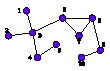
\includegraphics[width=\textwidth]{images/diffusion-graph.pdf}
			\caption{}
			\label{difn-graph}
		\end{subfigure}~
		\begin{subfigure}[b]{0.45\textwidth}
			\includegraphics[width= \textwidth]{images/simple-quantity-time.png}
			\caption{}
			\label{difn-plot}
		\end{subfigure}
		\caption{(\subref{difn-plot}) is an illustration of the diffusion process over the network in (\subref{difn-graph}). }
		\label{graph-plot}
	\end{figure}

%\begin{exa} Let us find out how the diffusion process occurs on a star network in Fig.~\ref{stargraph-plot}(\subref{stardifn-graph}). Consider the initial quantity of heat at the nodes be $\boldsymbol{\phi}(0)=[0.8,0,0,0,0,0,0,0,0,0]$ and let $C=0.5$.

Let us consider two other networks of different structures that is a star network and a regular network. We explore how diffusion occurs on networks of different structures and what impact the structure of the network has on the diffusion of a network.\\
To begin with, taking a star network in Fig.~\ref{stargraph-plot}(\subref{stardifn-graph}). Suppose the initial quantity of heat at the nodes is $\boldsymbol{\phi}(0)=[3,0,8,0,5,2,0,0,0,2]$ and let $C=1$. The spread of heat over the network is illustrated in Fig.~\ref{stargraph-plot}(\subref{stardifn-plot}).We observe that the quantity of heat at node $1$ (central node)drops so fast. This is because node $1$, which initially has the highest amount of heat, is directly connected to many other nodes whose heat contents are very low. Thus, node $1$ plays a central role in the exchange of heat within its neighborhood. The neighboring nodes to node $1$ which had no heat initially, steadily gain equal amounts of heat from node $1$ and as such their heat content raises as time goes by until the equilibrium point is reached. At $t=6$, the quantity of heat at all nodes is the same, that is, $\phi_j(6)= 1.6$ which implies equilibrium is attained for all nodes in the network.

For the $4$-regular network shown in Fig.~\ref{reggraph-plot}(\subref{regdifn-graph}).Suppose we set initial heat quantities as in the star network and with the same diffusion constant,we illustrate the diffusion process by Fig.~\ref{reggraph-plot}(\subref{regdifn-plot}). We observe that diffusion occurs much faster than in the star network that is to say by $t=2$, nodes are already tending to equilibrium point.

\begin{figure}[!h]
	\centering
	\begin{subfigure}[b]{0.27\textwidth}
		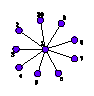
\includegraphics[width=\textwidth]{images/star-difusion.pdf}
		\caption{}
		\label{stardifn-graph}
	\end{subfigure}~
	\begin{subfigure}[b]{0.45\textwidth}
		\includegraphics[width= \textwidth]{images/star-quantity-time.png}
		\caption{}
		\label{stardifn-plot}
	\end{subfigure}
	\caption{(\subref{stardifn-plot}) is an illustration of the diffusion process over a star network in (\subref{stardifn-graph}). }
	\label{stargraph-plot}
\end{figure}

\begin{figure}[!h]
	\centering
	\begin{subfigure}[b]{0.27\textwidth}
		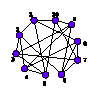
\includegraphics[width=\textwidth]{images/regular-dif.pdf}
		\caption{}
		\label{regdifn-graph}
	\end{subfigure}~
	\begin{subfigure}[b]{0.45\textwidth}
		\includegraphics[width= \textwidth]{images/regular-quantity-time.png}
		\caption{}
		\label{regdifn-plot}
	\end{subfigure}
	\caption{(\subref{regdifn-plot}) is an illustration of the diffusion process over a $4$-regular network in (\subref{regdifn-graph}). }
	\label{reggraph-plot}
\end{figure}

%\end{exa}

%\begin{exa} Let us explore how diffusion occurs on a regular network in Fig.~\ref{reggraph-plot}(\subref{regdifn-graph}). We set $\boldsym8bol{\phi}(0)= [0.3,0.0,0.8,0,0.5,0,0,0,0,0]$ and $C=0.5$. Fig.~\ref{stargraph-plot}(\subref{regdifn-plot}) illustrates the diffusion process over the network.  
% \end{exa}

A better visualisation of the diffusion process over the network in Fig.~\ref{graph-plot}(\subref{difn-graph}) at different time intervals is illustrated in Fig.~\ref{visualise} where the quantity of heat at any node at time $t$ is proportional to the size of the node.

\begin{figure}[!h]
	\centering
	\begin{subfigure}[b]{0.38\textwidth}
		\includegraphics[width=\textwidth]{images/newdiff-nodesize0.png}
		\caption{$t=0$}
		\label{t1}
	\end{subfigure}~
	\begin{subfigure}[b]{0.38\textwidth}
		\includegraphics[width= \textwidth]{images/newdiff-nodesize4.png}
		\caption{$t=3$}
		\label{t2}
	\end{subfigure}\\
	\begin{subfigure}[b]{0.38\textwidth}
		\includegraphics[width=\textwidth]{images/newdiff-nodesize14.png}
		\caption{$t=6$}
		\label{t3}
	\end{subfigure}~
	\begin{subfigure}[b]{0.38\textwidth}
		\includegraphics[width= \textwidth]{images/newdiff-nodesize29.png}
		\caption{$t=9$}
		\label{t4}
	\end{subfigure}
	\caption{Illustration of the diffusion process on a simple network in Fig.~\ref{graph-plot}(\subref{difn-graph}). Initially(t=0), all nodes are assigned certain quantities of heat according to the vector $\mathbf{\phi_0} = [3,0,8,0,5,2,0,0,0,2]$ where by the size of the node is proportional to the heat quantity that node has. Figures \ref{t1}, \ref{t2}, \ref{t3}, and \ref{t4} depict the status of the networks at $t=1$, $t=3$, $t=6$, and $t=9$ respectively. }
	\label{visualise}
\end{figure}


% Fig.~\ref{graph-plot}(\subref{difn-plot}), Fig.~\ref{stargraph-plot}(\subref{stardifn-graph}), and Fig.~\ref{reggraph-plot}(\subref{regdifn-plot}) illustrate how the diffusion processes occurs over different networks. 
In conclusion, we can tell that the structure of a network, the centralities of nodes, and the initial distribution of heat over a network play a key role in the diffusion process and hence have an impact on when diffusion is reached. For instance, equilibrium is reached faster in the star network as compared to the other two networks because the  most central node of the star network (node $1$) exchanges heat with its neighbors at a fast rate until equilibrium is reached.
  







%In this work, we consider diffusion of heat over a connected simple network where initial quantities of heat are generated and assigned randomly to nodes in the network at time $t=0$. We then study how heat spreads through the network until equilibrium is reached (i.e when all nodes in the network have equal temperatures). \\\\
%
%First, we consider direct flow of heat from one to only its neighbours. This literally means that a node can only spread or receive heat to or from nodes to which it is connected by a link.\\\\
\section{Diffusion on network with long range interactions}
In this case, we consider diffusion in a network where by both direct and long range interactions are involved. The long range interaction between two nodes $i$ and $j$ is determined by the length of the shortest path $d_{i,j}$ between nodes and the parameter $x$ ($0 \leq x < 0.5$). Thus, for any two that are not neighbours, we quantify long range interaction between them as $d_{i,j} x^{d_{i,j}-1}$.
%Secondly, we consider spread that involves not only direct connections among nodes but also long range interactions. 
For a simple undirected network with $n$ nodes,   
In case we consider a generalised adjacency matrix $A_{ij}(x)$ given by\\

\begin{equation*}
A_{i,j}(x) =  
\begin{cases} 
1 &\text{ if } \quad   i \sim j\\
d_{ij} x^{d_{ij}-1} & \text{ if } \quad   i\nsim j \quad  \&  \quad i\neq j \\
0 & \text{ if } \quad  i = j,
\end{cases}
\end{equation*}
where $d_{ij}$ is the shortest distance between nodes $i$ and $j$ and  $x$ is referred to as the conductance such that $0 \leq x < 0.5$.\\
Taking into account both direct and long range interactions (introducing conductance $x$), the rate of change in heat quantities for a given node $i$ over a change in time is given as 
\begin{eqnarray*}
\frac{d\phi_{i}(x)}{dt} &=& C \sum_{j} A_{i,j}(x) (\phi_j - \phi_i)\\
\frac{d\phi_{i}(x)}{dt} &=& C \sum_{j} A_{i,j}(x) \phi_j - C \phi_i \sum_{j} A_{i,j}(x)\\
\frac{d\phi_{i}(x)}{dt} &=& C \sum_{j} A_{i,j}(x) \phi_j - C \phi_i k_{i}(x)\\
\frac{d\phi_{i}(x)}{dt} &=& C \sum_{j} (A_{i,j}(x) - \delta_{i,j} k_{i}(x)) \phi_j
\end{eqnarray*}
In matrix notation;
\begin{equation}
\frac{d\phi(x)}{dt} + CL(x) \phi(x) = 0, \quad \phi(0,x) = \phi(0) = \phi_{0} ,
\label{eqn1}
\end{equation}
whose solution is
\begin{equation*}
\phi(t,x)  = \phi_0 \text{  } e^{-CL(x)t}
\end{equation*}
On the other hand, the solution can be expressed as a linear combination of eigenvectors $v_{i}(x)$ of $L(x)$ \\
\begin{equation*}
\phi(t,x)  = \sum_i a_{i}(t,x) v_{i} (x)
\end{equation*}
Substituting for $\phi_{i}(x)$ in \ref{eqn1}, we have
\begin{equation*}
\frac{d a_{i}(t,x)}{dt} + C\lambda_{i}(x) a_{i}(x) = 0, \quad i = 1, \hdots, n.
\end{equation*}
whose solution is\\
\begin{equation}
a_{i}(t,x) = a_{i}(0,x) e^{-C \lambda_{i}(x) t}
\label{eqn:2}
\end{equation}
Thus,
\begin{equation*}
\phi(t,x) = \sum_{i} a_{i}(0,x) \text{ } e^{-C \lambda_{i}(x) t} \mathbf{v_{i}(x)}
\end{equation*}
where\\
\begin{equation*}
a_{i}(0,x) = \langle \phi(0), \mathbf{v_{i}(x)}\rangle
\end{equation*}
Therefore given eigenvalues of $L(x)$ and their corresponding eigenvectors along with the initial heat quantities at each node $\phi_0$, we can compute the quantity at each node at a particular time $t$.\\\\
As time tends to infinity, we  can tell from eqn \ref{eqn:2} that equilibrium behaviour can be attained because the eigenvalues of the laplacian matrix $L(x)$ at conductance $x$ are non negative values which implies that the solution to eqn \ref{eqn:2} only decays exponentially or remains constant. However, it is important to note that rate of exponential decay is relatively faster when long range interactions are involved. This is because the eigenvalues $\lambda(x)$ are increasing functions of $x$ implying that $\lambda(x) \geq \lambda$. So we have
\begin{equation*}
\lim_{t \longrightarrow \infty}\text{ } e^{-C \lambda_{i}(x) t} = 
\begin{cases} 
0 \text{ if } & \lambda_{i}(x) > 0\\
1 \text{ if } & \lambda_{i}(x) = 0
\end{cases}
\end{equation*}
This implies that for $\lim_{t \longrightarrow \infty}$, the solution to eqn \ref{eqn:2} is  $a_{i}(0,x) e^{-C \lambda_{i}(x) t}$ for $\lambda_{i}=0$.
In other words, the equilibrium state of the system is completely determined by the kernel ($ker(L(x))= \{ \mathbf{v} \in \mathbf{V} | \mathbf{L}(x,\mathbf{v}) = \mathbf{0} \}$) of the $L(x)$. One of the vectors in $ker(L(x))$ is the all ones vector $\mathbf{v^1}$ since $\sum_j L_{i,j} (x) = 0$.\\
So for a graph with $n$ nodes and initial heat quantities  $phi_i$ at each node $i$, equilibrium behaviour is given by
\begin{equation*}
\lim_{t \longrightarrow \infty} \phi(t,x) = \langle \mathbf{\phi_0}, \mathbf{v(x) ^1}\rangle \mathbf{v(x)^1}
\end{equation*}
The quantity of heat $\phi_{j} (t,x)$ at any node $j$ at time $t$ when $x$ is introduced is given by\\
\begin{equation*}
\lim_{t \longrightarrow \infty} \phi_{j}(t,x) = \frac{1}{n} \sum_{i=1}^{n} \phi_{i} (0)
\end{equation*}

\section{Diffusion with long range Interactions for different Network structures}
Here we consider two networks that is Barabasi-Albert network whose degree distribution follows a power law and the other is the Erdos-Renyi network whose degree distribution follows exponential distribution. Both networks have $1000$ nodes and average degree $6$. We then investigate diffusion over the two networks for different values $x$ and results illustrated in Fig \ref{barabasi-Erdos-compare}.

\begin{figure}[!h]
	\centering
	\begin{subfigure}[b]{0.45\textwidth}
		\includegraphics[width=\textwidth]{images/barabasi-x0.png}
		\caption{$x=0$}
		\label{barabasi-x0}
	\end{subfigure}~
	\begin{subfigure}[b]{0.45\textwidth}
		\includegraphics[width= \textwidth]{images/erdos-x0.png}
		\caption{$x=0$}
		\label{erdos-x01}
	\end{subfigure}\\
	\begin{subfigure}[b]{0.45\textwidth}
		\includegraphics[width= \textwidth]{images/barabasi-x02.png}
		\caption{$x=0.2$}
		\label{barabasi-x02}
	\end{subfigure}~
	\begin{subfigure}[b]{0.45\textwidth}
		\includegraphics[width= \textwidth]{images/erdos-x02.png}
		\caption{$x=0.2$}
		\label{erdos-x02}
	\end{subfigure}\\
	\begin{subfigure}[b]{0.45\textwidth}
		\includegraphics[width= \textwidth]{images/barabasi-x04.png}
		\caption{$x=0.4$}
		\label{barabasi-x04}
	\end{subfigure}~
	\begin{subfigure}[b]{0.45\textwidth}
		\includegraphics[width= \textwidth]{images/erdos-x04.png}
		\caption{$x=0.4$}
		\label{erdos-x04}
	\end{subfigure}
	\caption{Barabasi networks (left) and Erdos Renyi networks(right) of 1000 nodes and average degree of 6. Top row is illustration of diffusion process at $x=0$ ( i.e accounting for direct interactions only), middle row corresponds to $x=0.2$ followed by $x=0.4$ in the last row}
	\label{barabasi-Erdos-compare}
\end{figure}

From Fig \ref{barabasi-Erdos-compare} at the top row, we observe that at $x=0$, equilibrium is reached faster for Barabasi-Alberto(BA) network ( that is after about $4$ time steps) compared to Erdos-Renyi(ER) network in which equilibrium is reached after about $10$ time steps. This is explained based on the fact that in BA networks there are more hubs compared to ER networks. These hubs tend to interact with a number of nodes with in the network thus fastening the diffusion process. On increasing $x$ to $0.2$, we observe a drastic drop in equilibrium time from  $4$ to $0.15$ time steps and from $10$ to $0.8$ time steps for BA and ER networks respectively. It is important to note that drop in equilibrium time is relatively higher in ER than in BA and this is because of the few hubs in ER networks which aids a larger number of long range interactions than in BA networks. As $x$ increases further to $0.4$, equilibrium time further drops to $0.03$ and $0.06$ for BA and ER networks respectively.

\section{Degree Centrality and Diffusion on networks}
%We take a Barabasi-Albert network and Erdos-Renyi network, both of 100 nodes and average of 6. We choose $5$ nodes with the highest degree centrality to which we assign specific amounts of heat. At each time $t$, we measure the average quantity of heat at the $5$ nodes as illustrated by figure. 

\begin{figure}[!h]
	\centering
	\begin{subfigure}[b]{0.45\textwidth}
		\includegraphics[width= \textwidth]{images/barabasi-average.png}
		\caption{}
		\label{}
	\end{subfigure}~
	\begin{subfigure}[b]{0.45\textwidth}
		\includegraphics[width= \textwidth]{images/E-R-average.png}
		\caption{}
		\label{}
	\end{subfigure}
    \caption{ Results of the simulations for two networks. One is the Barabasi-Albert(BA) network and  the other is Erdos-Renyi(ER) network, both of $100$ nodes and average degree of $6$. Taking $5$ of the most important (by degree) nodes in the network from which diffusion is initiated by assigning certain quantities of heat to those nodes, the simulation of the diffusion is illustrated in plots (a) and (b) for the BA and ER networks respectively.}
    \label{key}
\end{figure}

We observe that in BA network, heat spreads quite faster than in ER network that is to say by $t=0.6$, all the $5$ hubs in BA have levelled to equal amount while for ER, nodes still have un equal amounts of heat. This is because we assign quantities of heat to $5$ hubs of a network and they quickly spread heat to other nodes compared to ER where there are relatively fewer hubs among the five chosen nodes to initiate the diffusion process.

\section{Diffusion process on a grid}
We consider a 2-dimensional discrete grid in which each point is connected to 8 of its nearest neighbours. Initially, we assign heat quantities to all the points on the grid and then we investigate how the diffusion process occurs and at each time $t$, we compute the quantity of heat at each node using equation \ref{dif-final-eqn}. \\
Let us take a 20 by 20 grid on which we assigned heat quantities of amounts 5, 7 and 10 to a few points and the rest are assigned zero. The figures below illustrate the diffusion process in which both the direct and long range interactions are accounted for at different values of x.
\begin{figure}[!h]
	\centering
	\begin{subfigure}[b]{0.25\textwidth}
		\includegraphics[width=\textwidth]{images/grid-t0-x0.png}
		%\caption{$x=0, t=0$}
		%\label{gridt0x0}
	\end{subfigure}~
	\begin{subfigure}[b]{0.25\textwidth}
		\includegraphics[width= \textwidth]{images/grid-t05-x0.png}
		%\caption{$x=0, t=0.5$}
		%\label{gridt05x01}
	\end{subfigure}~
    \begin{subfigure}[b]{0.25\textwidth}
    	\includegraphics[width= \textwidth]{images/grid-t3-x0.png}
    	%\caption{$x=0, t=3.0$}
    	%\label{gridt3x01}
    \end{subfigure}~
    \begin{subfigure}[b]{0.25\textwidth}
    	\includegraphics[width= \textwidth]{images/grid-t5-x0.png}
    	%\caption{$x=0, t=5.0$}
    	%\label{gridt5x01}
    \end{subfigure}
%\caption{Sample illustrations for progression of diffusion for $x=0$ i.e direct interactions only.}
%\label{gridatx0}
\end{figure}

\begin{figure}[!h]
	\centering
	\begin{subfigure}[b]{0.25\textwidth}
		\includegraphics[width=\textwidth]{images/grid-t0-x01.png}
		%\caption{$x=0.1, t=0$}
		%\label{gridt0x01}
	\end{subfigure}~
	\begin{subfigure}[b]{0.25\textwidth}
		\includegraphics[width= \textwidth]{images/grid-t05-x01.png}
		%\caption{}
		%\label{}
	\end{subfigure}~
	\begin{subfigure}[b]{0.25\textwidth}
		\includegraphics[width= \textwidth]{images/grid-t3-x01.png}
		%\caption{}
		%\label{}
	\end{subfigure}~
	\begin{subfigure}[b]{0.25\textwidth}
		\includegraphics[width= \textwidth]{images/grid-t5-x01.png}
		%\caption{}
		%\label{}
	\end{subfigure}
\end{figure}

\begin{figure}[!h]
	\centering
	\begin{subfigure}[b]{0.25\textwidth}
		\includegraphics[width=\textwidth]{images/grid-t0-x02.png}
		%\caption{$x=0.2, t=0$}
		%\label{gridt0x02}
	\end{subfigure}~
	\begin{subfigure}[b]{0.25\textwidth}
		\includegraphics[width= \textwidth]{images/grid-t05-x02.png}
		%\caption{$x=0.2, t=0.5$}
		%\label{gridt05x02}
	\end{subfigure}~
	\begin{subfigure}[b]{0.25\textwidth}
		\includegraphics[width= \textwidth]{images/grid-t3-x02.png}
		%\caption{$x=0.2, t=3.0$}
		%\label{gridt2x02}
	\end{subfigure}~
	\begin{subfigure}[b]{0.25\textwidth}
		\includegraphics[width= \textwidth]{images/grid-t5-x02.png}
		%\caption{$x=0.2, t=5.0$}
		%\label{gridt3x02}
	\end{subfigure}\\
\vspace{0.25cm}
	 \begin{subfigure}[b]{0.60\textwidth}
	 	\includegraphics[width= \textwidth]{images/colour-bar-grid.png}
	 \end{subfigure}
\caption{Illustrations for diffusion over a grid. The upper most row corresponds to diffusion when only direct interac tions among neighbouring nodes are accounted for. The middle and last row are results obtained when long range interactions are included at $x=0.1$ and $x=0.2$ respectively. The intensity of heat follows a color grid where by red implies higher intensity followed by yellow and blue implies low heat intensities.}
\label{diffusionongrid}
\end{figure}

At $t=0$, diffusion on the grid starts off with $3$ strong regions having high quantities of heat as observed from observe figures \ref{gridatx0}, \ref{gridatx01}, and \ref{gridatx02} which correspond to $x$ values of $0$, $0.1$ and $0.2$ respectively. As the diffusion process continues, we see that at $t=0.5$, strong heat points can still be spotted for $x=0$, relatively strong points in $x=0.1$ and almost complete diffusion in $x=0.2$. we can also see that by $t=2.0$, heat is uniformly distributed across the grid for $x=0.1$ and $x=0.2$. However, for $x=0$ diffusion is still ongoing and we can notice strong heat points at the centre of the grid. Following the sequences in the figures, we can conclude that as $x$ (i.e increase in intensity of long range interactions), the diffusion process goes faster and equilibrium across the grid is reached faster as observed in the above simulations where for $x=0.2$,$x=0.1$ equilibrium is reached by $t=3$ while for $x=0$, equilibrium is not yet reached by then.


%%%otherwork%%%%
%Here we investigate diffusion of heat over a given network. First we consider heat transfer through short range interactions and later introduce long range interactions by tuning the conductance, 
%$x [0 <= x< 0.4]$
%Consider a  simple network (shown in Fig below) with $10$ nodes and initial heat quantities $Q_0 = [3.0, 0.0, 8.0 ,0 .0, 5.0 , 2.0 , 0.0 ,0.0 ,0.0, 2.0]$. Let the diffusion constant, $C= 1$. We then find out how long it takes for all nodes in the network to reach equilibrium for different values of conductance $x$.
%
%\begin{figure}[!h]
%	\centering
%	\includegraphics[width=0.5\textwidth]{images/star-longandshort.png}
%	\caption{star network of size $10$}
%	\label{starlongandshort}
%\end{figure}
%
%\begin{figure}[!h]
%	\centering
%	\begin{subfigure}[b]{0.38\textwidth}
%		\includegraphics[width=\textwidth]{images/star-longandshortx0.png}
%		\caption{$x=0$}
%		\label{star-longandshortx0}
%	\end{subfigure}~
%	\begin{subfigure}[b]{0.38\textwidth}
%		\includegraphics[width= \textwidth]{images/star-longandshortx01.png}
%		\caption{$x=0.1$}
%		\label{star-longandshortx0}
%	\end{subfigure}\\
%	\begin{subfigure}[b]{0.38\textwidth}
%		\includegraphics[width=\textwidth]{images/star-longandshortx02.png}
%		\caption{$x=0.2$}
%		\label{t3}
%	\end{subfigure}~
%	\begin{subfigure}[b]{0.38\textwidth}
%		\includegraphics[width= \textwidth]{images/star-longandshortx03.png}
%		\caption{$x=0.3$}
%		\label{star-longandshortx03}
%	\end{subfigure}
%	\caption{Illustration of the diffusion process at different time intervals over the network in Fig.~\ref{graph-plot}(\subref{difn-graph}).}
%	\label{visualise}
%\end{figure}
%From the Figures above we observe that, considering only short range interactions among nodes, equilibrium is reached at $T=48$. As we introduce long range interactions, at $x=0.1$, Equilibrium is reached much faster , $T= 20$ ( less then half the time it takes when only short range interactions are considered). As we increase the conductance we observe faster diffusion process that is to say at $x=0.2$ and $x=0.3$, equilibrium is obtained at $T=10$ and $T=5$ respectively. For every increase in conductance by $0.1$, the time at which equilibrium is achieved is halved.
%
%Lets investigate the impact of the structure of a network on the diffusion of heat over a network for different values of conductance. 
%
%Path Network (shown in Figure below ) has $10$ nodes and same initial heat distribution as the network above. Nodes $1,3,5,6,$ and $10$ are assigned initial quantities of $3, 8, 5, 2 and 2$ respectively while the rest of the nodes are assigned $0$.
%
%\begin{figure}[!h]
%	\centering
%	\includegraphics[width=0.5\textwidth]{images/path-longandshort.png}
%	\caption{star network of size $10$}
%	\label{starlongandshort}
%\end{figure}
%
%\begin{figure}[!h]
%	\centering
%	\begin{subfigure}[b]{0.38\textwidth}
%		\includegraphics[width=\textwidth]{images/path-longandshortx0.png}
%		\caption{$x=0$}
%		\label{star-longandshortx0}
%	\end{subfigure}~
%	\begin{subfigure}[b]{0.38\textwidth}
%		\includegraphics[width= \textwidth]{images/path-longandshortx01.png}
%		\caption{$x=0.1$}
%		\label{star-longandshortx0}
%	\end{subfigure}\\
%	\begin{subfigure}[b]{0.38\textwidth}
%		\includegraphics[width=\textwidth]{images/path-longandshortx02.png}
%		\caption{$x=0.2$}
%		\label{t3}
%	\end{subfigure}~
%	\begin{subfigure}[b]{0.38\textwidth}
%		\includegraphics[width= \textwidth]{images/path-longandshortx0.png}
%		\caption{$x=0.3$}
%		\label{star-longandshortx03}
%	\end{subfigure}
%	\caption{Illustration of the diffusion process at different time intervals over the network in Fig.~\ref{graph-plot}(\subref{difn-graph}).}
%	\label{visualise}
%\end{figure}
%
%At conductance, $x=0$,  Equilibrium is reached time $T=100$ ( far longer than in the previous network),   and as we vary the conductance from $0.1$ through $0.3$, there is a reduction in the time required for equilibrium to be attained i.e. 45, 25 and 15 respectively. 
%
%STAR NETWORK:
%
%Consider a star graph of the same size (10) as the previous graphs and with similar initial heat allocations.  The figure at the right illustrates different times at which equilibrium of all nodes is attained at varying conductance values.
%\begin{figure}[!h]
%	\centering
%	\begin{subfigure}[b]{0.38\textwidth}
%		\includegraphics[width=\textwidth]{images/star-combined.png}
%		\caption{Star Network}
%		\label{star-combined}
%	\end{subfigure}~
%	\begin{subfigure}[b]{0.38\textwidth}
%		\includegraphics[width= \textwidth]{images/star-combined-plot.png}
%		\caption{Combined plot}
%		\label{star-combined-plot}
%	\end{subfigure}	
%	\caption{Illustration of the diffusion process at different time intervals over the network in Fig.~\ref{graph-plot}(\subref{difn-graph}).}
%	\label{visualise}
%\end{figure}
%With only short range interactions (at $x=0$), equilibrium is reached faster than in path network (i.e at $T=11$). This is very fast compared to the two networks discussed before. As the conductance is increased, the time rapidly reduces to $T=4, T=2.5, T=2.0$ and $T=1.5$ for $x=0.1,0.2,0.3$ and $0.4$ respectively.
%
%LATTICE:
%
%\begin{figure}[!h]
%	\centering
%	\includegraphics[width=0.5\textwidth]{images/lattice.png}
%	\caption{Lattice of size $10$}
%	\label{starlongandshort}
%\end{figure}
%
%
%
%\begin{figure}[!h]
%	\centering
%	\begin{subfigure}[b]{0.38\textwidth}
%		\includegraphics[width=\textwidth]{images/latticex0.png}
%		\caption{$x=0$}
%		\label{star-longandshortx0}
%	\end{subfigure}~
%	\begin{subfigure}[b]{0.38\textwidth}
%		\includegraphics[width= \textwidth]{images/latticex01.png}
%		\caption{$x=0.1$}
%		\label{star-longandshortx0}
%	\end{subfigure}\\
%	\begin{subfigure}[b]{0.38\textwidth}
%		\includegraphics[width=\textwidth]{images/latticex02.png}
%		\caption{$x=0.2$}
%		\label{t3}
%	\end{subfigure}~
%	\begin{subfigure}[b]{0.38\textwidth}
%		\includegraphics[width= \textwidth]{images/latticex03.png}
%		\caption{$x=0.3$}
%		\label{star-longandshortx03}
%	\end{subfigure}
%	\caption{Illustration of the diffusion process at different time intervals over the network in Fig.~\ref{graph-plot}(\subref{difn-graph}).}
%	\label{visualise}
%\end{figure}
%
%Diffusion over a lattice occurs quite faster than in a path network, We see from the above illustrations that at x=0, equilibrium is attained at T= 22 compared to that of the path network which was at T=100. However, this is slower compared to star network. As conductance increases to x=0.1, we observe a drop in time to T=10 followed by T=6 and T= 4 for x= 0.2 and x=0.3 respectively. 
%
%
%\begin{figure}[!h]
%	\centering
%	\begin{subfigure}[b]{0.38\textwidth}
%		\includegraphics[width=\textwidth]{images/comparisonx0.png}
%		\caption{$x=0$}
%		\label{comparisonx0}
%	\end{subfigure}~
%	\begin{subfigure}[b]{0.38\textwidth}
%		\includegraphics[width= \textwidth]{images/comparisonx01.png}
%		\caption{$x=0.1$}
%		\label{comparisonx01}
%	\end{subfigure}\\
%	\begin{subfigure}[b]{0.38\textwidth}
%		\includegraphics[width=\textwidth]{images/comparisonx02.png}
%		\caption{$x=0.2$}
%		\label{comparisonx02}
%	\end{subfigure}~
%	\begin{subfigure}[b]{0.38\textwidth}
%		\includegraphics[width= \textwidth]{images/comparisonx03.png}
%		\caption{$x=0.3$}
%		\label{comparisonx03}
%	\end{subfigure}
%	\caption{Illustration of the diffusion process at different time intervals over the network in Fig.~\ref{graph-plot}(\subref{difn-graph}).}
%	\label{visualise}
%\end{figure}
%
%BARABASI Network
%
%Using networkx, we create the Barabasi with 100 number of nodes and  m edges to attach  from a new node to existing nodes. (Average degree $\sim 6$)
%
%\begin{figure}[!h]
%	\centering
%	\includegraphics[width=0.5\textwidth]{images/barabasi.png}
%	\caption{Lattice of size $10$}
%	\label{barabasi}
%\end{figure}
%
%
%\begin{figure}[!h]
%	\centering
%	\begin{subfigure}[b]{0.38\textwidth}
%		\includegraphics[width=\textwidth]{images/barabasix0.png}
%		\caption{$x=0$}
%		\label{barabasix0}
%	\end{subfigure}~
%	\begin{subfigure}[b]{0.38\textwidth}
%		\includegraphics[width= \textwidth]{images/barabasix01.png}
%		\caption{$x=0.1$}
%		\label{barabasix01}
%	\end{subfigure}\\
%	\begin{subfigure}[b]{0.38\textwidth}
%		\includegraphics[width=\textwidth]{images/barabasix02.png}
%		\caption{$x=0.2$}
%		\label{barabasix02}
%	\end{subfigure}~
%	\begin{subfigure}[b]{0.38\textwidth}
%		\includegraphics[width= \textwidth]{images/barabasix03.png}
%		\caption{$x=0.3$}
%		\label{barabasix03}
%	\end{subfigure}
%	\caption{Illustration of the diffusion process at different time intervals over the network in Fig.~\ref{graph-plot}(\subref{difn-graph}).}
%	\label{visualise}
%\end{figure}
%
%ERDOS-RENYI RANDOM NETWORK:
%
%Using networkx, we create a random model with 100 nodes and with probability, p = 0.06 and average degree of  $\sim 6$.
%\begin{figure}[!h]
%	\centering
%	\begin{subfigure}[b]{0.38\textwidth}
%		\includegraphics[width=\textwidth]{images/comparisonx0.png}
%		\caption{$x=0$}
%		\label{comparisonx0}
%	\end{subfigure}~
%	\begin{subfigure}[b]{0.38\textwidth}
%		\includegraphics[width= \textwidth]{images/comparisonx01.png}
%		\caption{$x=0.1$}
%		\label{comparisonx01}
%	\end{subfigure}\\
%	\begin{subfigure}[b]{0.38\textwidth}
%		\includegraphics[width=\textwidth]{images/comparisonx02.png}
%		\caption{$x=0.2$}
%		\label{comparisonx02}
%	\end{subfigure}~
%	\begin{subfigure}[b]{0.38\textwidth}
%		\includegraphics[width= \textwidth]{images/comparisonx03.png}
%		\caption{$x=0.3$}
%		\label{comparisonx03}
%	\end{subfigure}
%	\caption{Illustration of the diffusion process at different time intervals over the network in Fig.~\ref{graph-plot}(\subref{difn-graph}).}
%	\label{visualise}
%\end{figure}
%
%BARABASI Network
%
%Using networkx, we create the Barabasi with 100 number of nodes and  m edges to attach  from a new node to existing nodes. (Average degree $\sim 6$)
%
%
%\begin{figure}[!h]
%	\centering
%	\begin{subfigure}[b]{0.38\textwidth}
%		\includegraphics[width=\textwidth]{images/randomx0.png}
%		\caption{$x=0$}
%		\label{randomx0}
%	\end{subfigure}~
%	\begin{subfigure}[b]{0.38\textwidth}
%		\includegraphics[width= \textwidth]{images/randomx01.png}
%		\caption{$x=0.1$}
%		\label{randomx01}
%	\end{subfigure}\\
%	\begin{subfigure}[b]{0.38\textwidth}
%		\includegraphics[width=\textwidth]{images/randomx02.png}
%		\caption{$x=0.2$}
%		\label{randomx02}
%	\end{subfigure}~
%	\begin{subfigure}[b]{0.38\textwidth}
%		\includegraphics[width= \textwidth]{images/randomx03.png}
%		\caption{$x=0.3$}
%		\label{randomx03}
%	\end{subfigure}
%	\caption{Illustration of the diffusion process at different time intervals over the network in Fig.~\ref{graph-plot}(\subref{difn-graph}).}
%	\label{visualise}
%\end{figure}
%
%
%
%For the Scale free Barabasi network and random E-R network of the same number of nodes 100 and  average degree k ~ 6.  We observe that at conductance x=0 (that is only short range interactions), diffusion occurs quite faster in BA network as compared to E-R network that is to say equilibrium for all nodes is attained at T= 6.5 and T=13.5 respectively.
%
%As we introduce conductance, x=0.1, equilibrium is attained at much faster in both cases but still BA networks reaches equilibrium faster than the random networks. This occurs at times T=1.5 and T=3.5 respectively.
%As the conductance increases, diffusion happens very fast that is equilibrium is reached almost immediately in Barabasi and in less than T=2 in random networks. 

\section{Previous Discussions}
\begin{figure}[!h]
	\centering
	\begin{subfigure}[b]{0.30\textwidth}
		\includegraphics[width=\textwidth]{images/quantity-time-exponents-x0.png}
		%\caption{$x=0.1, t=0$}
		%\label{gridt0x01}
	\end{subfigure}~
	\begin{subfigure}[b]{0.30\textwidth}
		\includegraphics[width= \textwidth]{images/quantity-time-exponents-x01.png}
		%\caption{$x=0.1, t=0.5$}
		%\label{gridt05x01}
	\end{subfigure}~
	\begin{subfigure}[b]{0.30\textwidth}
		\includegraphics[width= \textwidth]{images/quantity-time-exponents-x03.png}
		%\caption{$x=0.1, t=3.0$}
		%\label{gridt3x01}
	\end{subfigure}
	\caption{Plots of the average quantity of heat for $200$ nodes with the highest degree centrality against time for $3$ scale free networks having different values of the power exponent($2.0$,$2.3$,$2.7$, and $3.0$), n=1000 and average degree=$6$. The figures to the left, centre and right correspond to x values $0$,$0.1$, and $0.3$ respectively.}
	\label{gridatx01}
\end{figure}

\begin{figure}[!h]
	\centering
	\begin{subfigure}[b]{0.40\textwidth}
		\includegraphics[width=\textwidth]{images/Barabasi-highest-degree.png}
		%\caption{$x=0.1, t=0$}
		%\label{gridt0x01}
	\end{subfigure}~
	\begin{subfigure}[b]{0.40\textwidth}
		\includegraphics[width= \textwidth]{images/barabasi-random-selection.png}
		%\caption{$x=0.1, t=0.5$}
		%\label{gridt05x01}
	\end{subfigure}
	\caption{Illustration of the impact of the choice of the initial nodes from which diffusion starts. We consider Barabasi-Alberto networks of $100$ nodes. The left plot corresponds to one in which the $5$ most important node according to degree centrality(hubs) are chosen. On the other hand, the right plot is as a result of choosing the initial nodes randomly. }
	\label{}
\end{figure}


\begin{figure}[!h]
	\centering
	\begin{subfigure}[b]{0.32\textwidth}
		\includegraphics[width=\textwidth]{images/Simple-network-eigenplot.png}
		%\caption{$x=0.1, t=0$}
		%\label{gridt0x01}
	\end{subfigure}~
	\begin{subfigure}[b]{0.32\textwidth}
		\includegraphics[width= \textwidth]{images/Star-network-eigenplot.png}
		%\caption{$x=0.1, t=0.5$}
		%\label{gridt05x01}
	\end{subfigure}~
	\begin{subfigure}[b]{0.32\textwidth}
		\includegraphics[width= \textwidth]{images/Path-network-eigenplot.png}
		%\caption{$x=0.1, t=3.0$}
		%\label{gridt3x01}
	\end{subfigure} \\
    \begin{subfigure}[b]{0.85\textwidth}
    	\includegraphics[width= \textwidth]{images/legend-eigenvalues.png}
    	%\caption{$x=0.1, t=3.0$}
    	%\label{gridt3x01}
    \end{subfigure}
	\caption{Results showing variation of eigenvalues with $x$. From left to right is simple networks(Fig. \ref{difn-graph}), star network (in Fig. \ref{stardifn-graph}) and path network respectively. All networks consist of $10$ nodes.}
	\label{}
\end{figure}

%\clearpage
%\nocite{*}
%\bibliographystyle{abbrv}
%\bibliography{references}
\end{document}
